\documentclass[border=10pt]{standalone}
\usepackage{tikz}
\usepackage{pgfplots}
\pgfplotsset{compat=1.8}
% zooming
\usetikzlibrary{spy}

\begin{document}
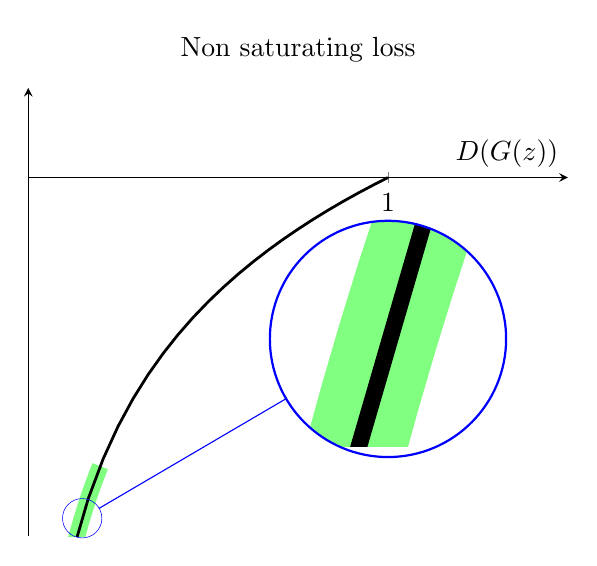
\begin{tikzpicture}[spy using outlines=
{circle, magnification=6, connect spies}]
	\begin{axis}[
		xlabel=$D(G(z))$,
		xmin=0,
		xmax=1.5,
		ymin = -2,
		ymax=0.5,
		axis lines=middle,
		ylabel near ticks,
		xtick={0,1},
		ytick=\empty,
		title={Non saturating loss}
	]
	
	% shading
	\addplot[line width=6pt,color = green!50, domain = 0:0.2]
	{ln(x)};
	
	% use TeX as calculator:
	\addplot [mark=none,domain=0:1, line width=1pt] {ln(x)};
	
	\coordinate (spypoint) at (axis cs:0.15,-1.9);
	\coordinate (magnifyglass) at (axis cs:1,-0.9);

	
	\end{axis}
	
	\spy [blue, size=3cm] on (spypoint)
	in node[fill=white] at (magnifyglass);
\end{tikzpicture}

\end{document}